\documentclass[11pt,a4paper]{article}

% --- Basic Packages ---
\usepackage[utf8]{inputenc}
\usepackage[T1]{fontenc}
\usepackage{graphicx}       
\usepackage{geometry}       
\usepackage{float}          
\usepackage{caption}        
\usepackage{hyperref}       
\usepackage{booktabs}       
\usepackage{amsmath}

\geometry{margin=1in}

% --- Title Information ---
\title{Performance Comparison of Stochastic Optimization Algorithms \\ \large Analysis of GD, SGD, Adam, SVRG, and MB-SVRG}
\author{Experimental Report}
\date{\today}

\begin{document}

\maketitle

\section{Experimental Overview}
This report evaluates the performance of various optimization algorithms across different datasets and architectures.
\begin{itemize}
    \item \textbf{Datasets:} California Housing (Regression), MNIST (Classification), and CIFAR-10 (Classification).
    \item \textbf{Model Architectures:} Linear Model, MLP-1 (1 hidden layer), and MLP-3 (3 hidden layers).
    \item \textbf{Evaluation Metrics:} Training Loss ($P(w)$), Test Error (RMSE or 1-Accuracy), and Gradient Variance Proxy (Rolling Standard Deviation of Loss).
\end{itemize}

% --- California Housing Section ---
\newpage
\section{Dataset: California Housing (Regression)}
This task utilizes the Mean Squared Error (MSE) loss function. Due to the high dynamic range of gradients in regression tasks, it poses a significant challenge to the stability of first-order optimizers.

\begin{figure}[H]
    \centering
    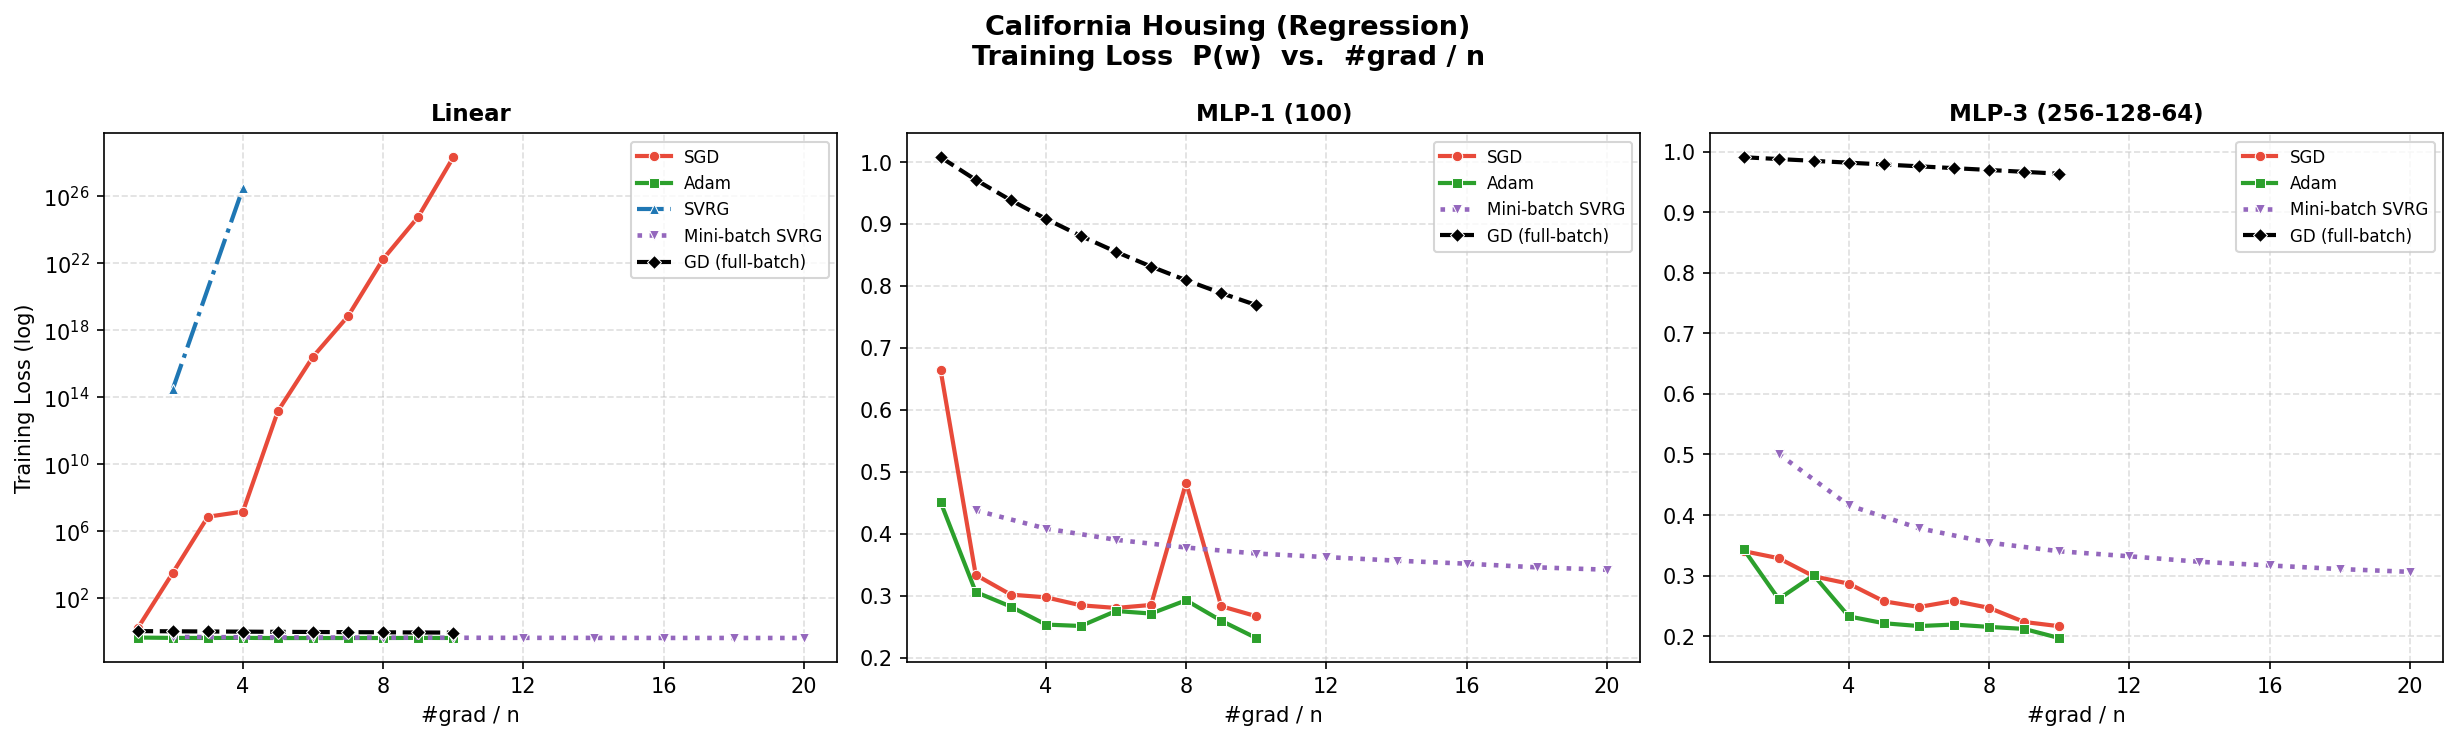
\includegraphics[width=1.0\textwidth]{plots/california_housing_1_train_loss_vs_gradn.png}
    \caption{California Housing: Training Loss Comparison (Left: Linear, Middle: MLP-1, Right: MLP-3)}
\end{figure}

\begin{figure}[H]
    \centering
    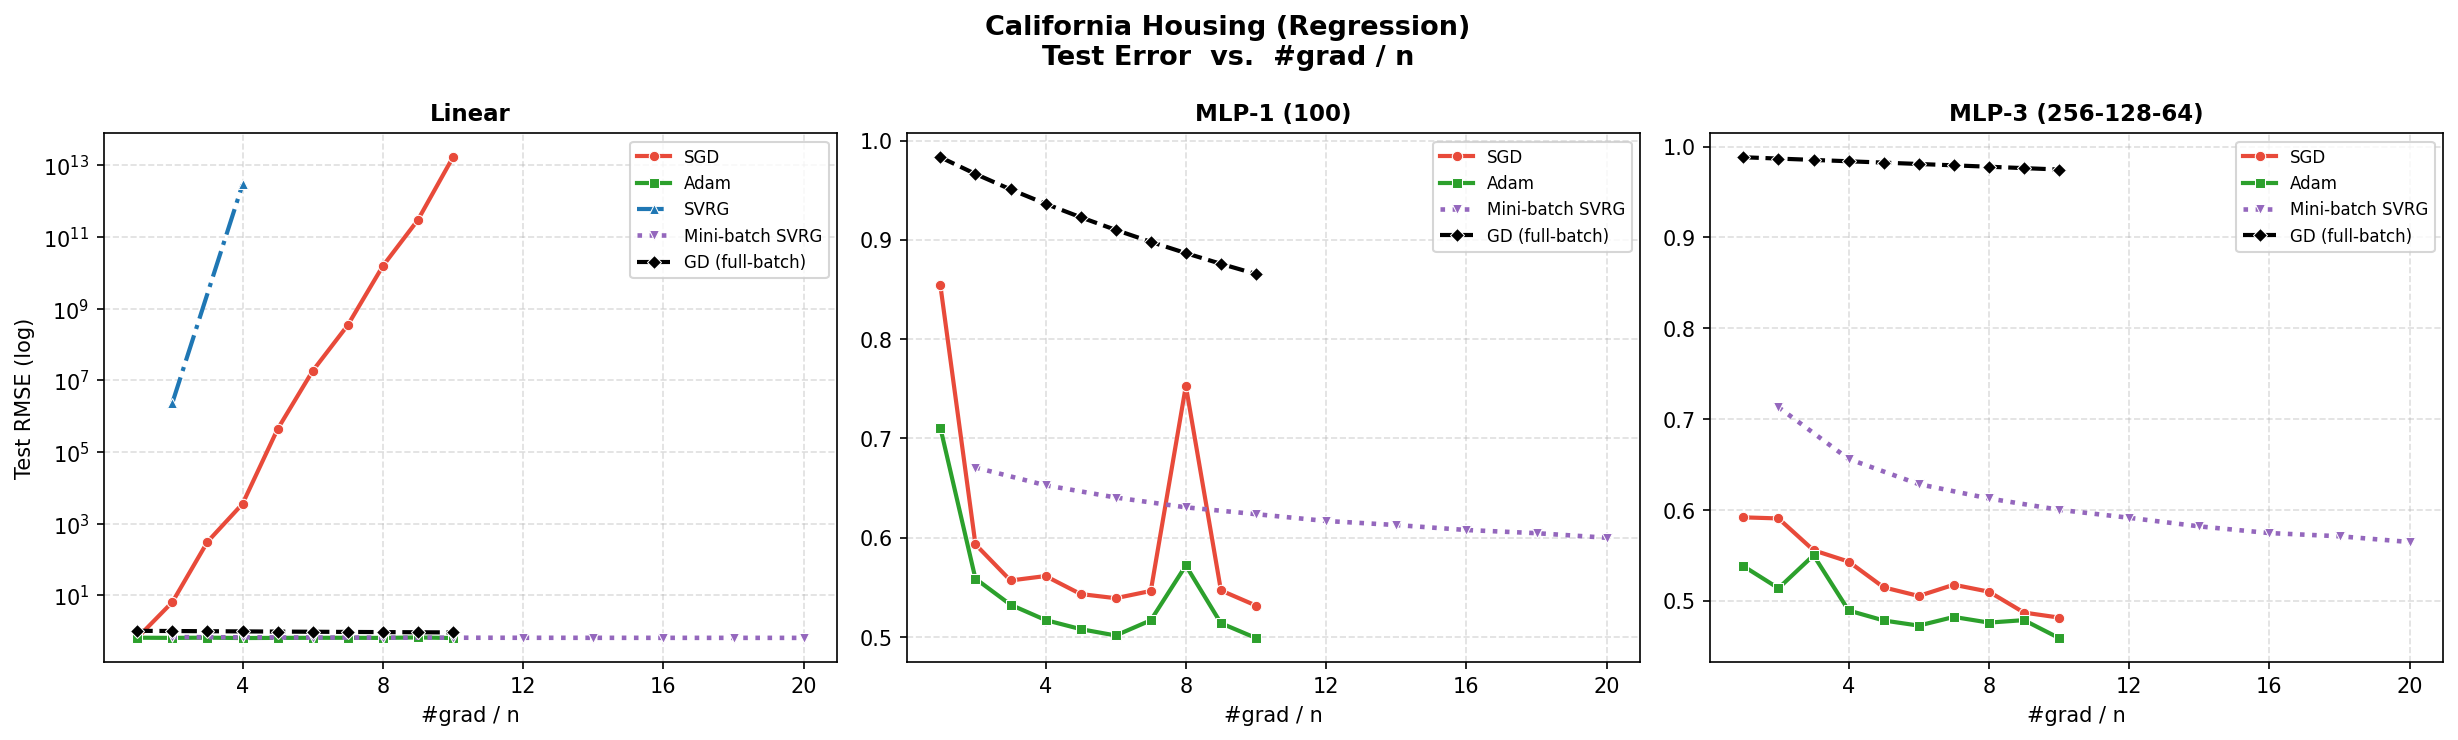
\includegraphics[width=1.0\textwidth]{plots/california_housing_2_test_error_vs_gradn.png}
    \caption{California Housing: Test Error (RMSE) Comparison}
\end{figure}

\begin{figure}[H]
    \centering
    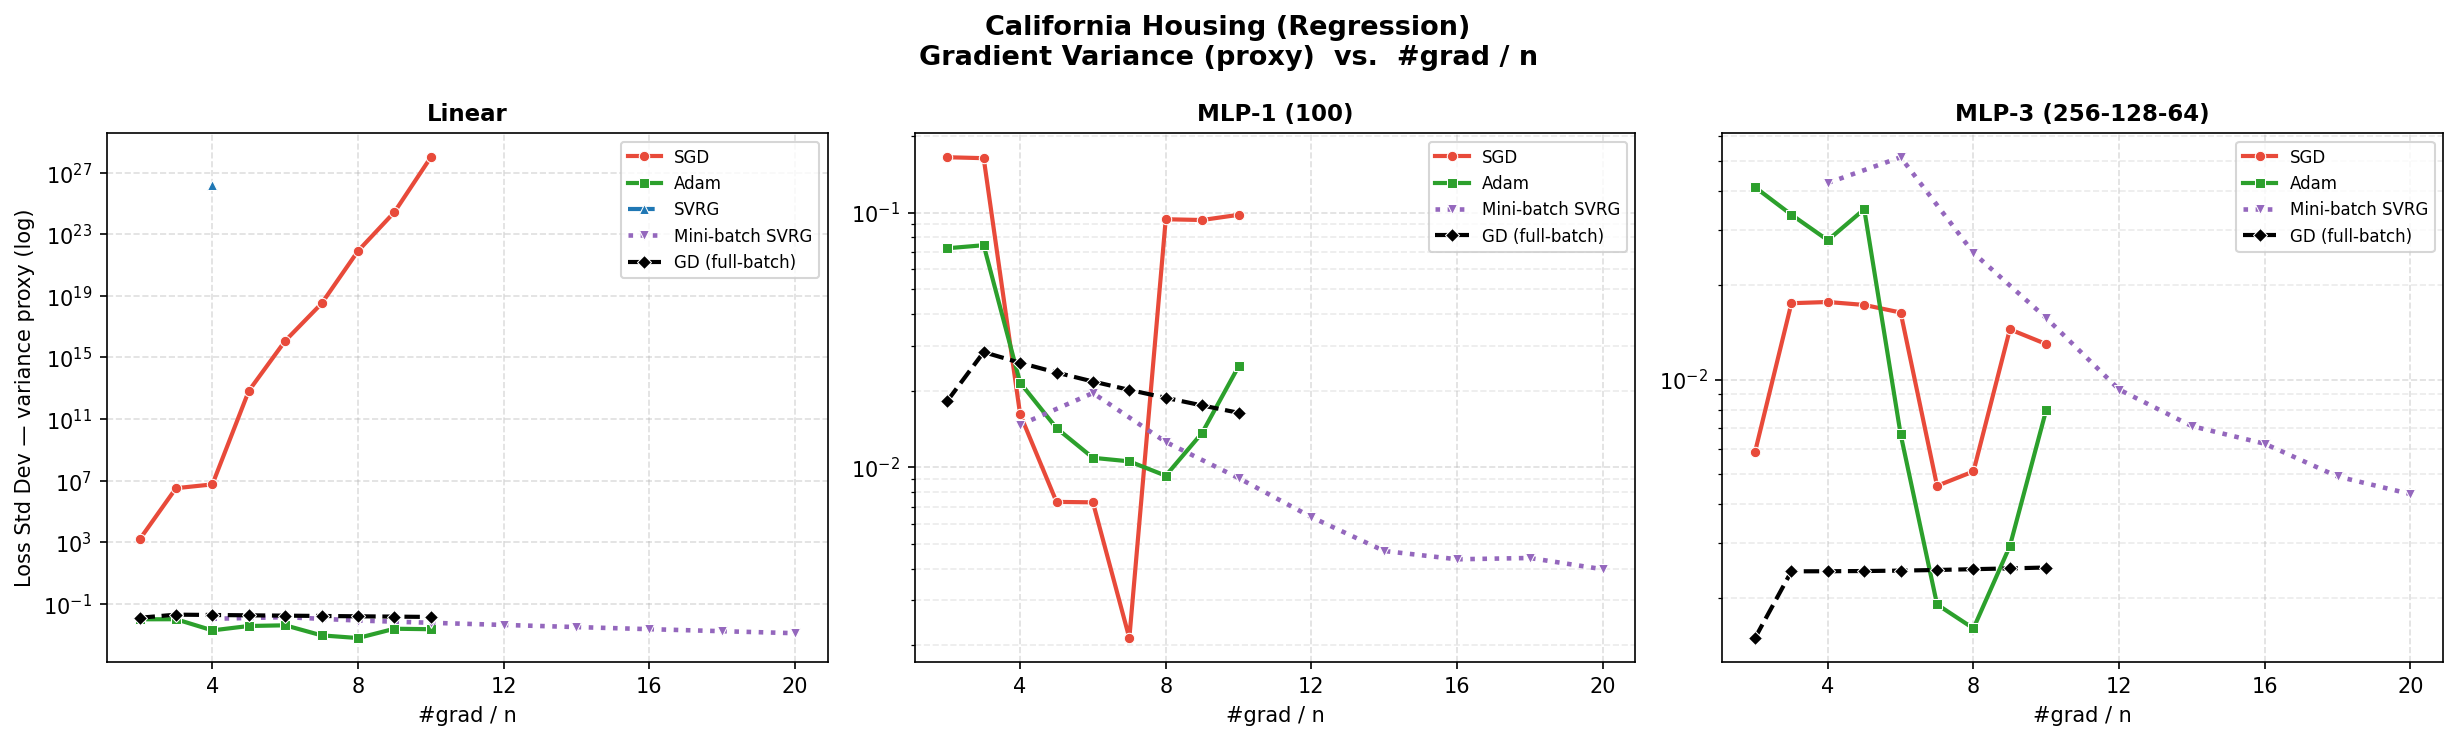
\includegraphics[width=1.0\textwidth]{plots/california_housing_3_variance_vs_gradn.png}
    \caption{California Housing: Gradient Variance Proxy Comparison}
\end{figure}

\subsection{Mathematical Analysis of Regression Results}

The California Housing task is a regression problem using the Mean Squared Error (MSE) loss function:
\begin{equation}
P(w) = \frac{1}{n} \sum_{i=1}^{n} \frac{1}{2} \| \phi(x_i; w) - y_i \|^2
\end{equation}
where $\phi(x_i; w)$ represents the model prediction. The gradient for a single sample $i$ is:
\begin{equation}
\nabla \psi_i(w) = (\phi(x_i; w) - y_i) \cdot \nabla_w \phi(x_i; w)
\end{equation}

\subsubsection{Why SGD and SVRG Diverge (Gradient Explosion)}
In the Training Loss plot, we observe that SGD (red) and SVRG (blue) exhibit catastrophic divergence ($Loss > 10^{10}$). Mathematically, for a gradient descent step $w_{t+1} = w_t - \eta \nabla \psi_i(w_t)$ to converge, the learning rate $\eta$ must satisfy:
\begin{equation}
\eta < \frac{2}{\lambda_{max}(H)}
\end{equation}
where $\lambda_{max}(H)$ is the largest eigenvalue of the Hessian matrix. In MSE regression, the gradient magnitude is directly proportional to the residual $(\phi(x_i; w) - y_i)$. 

Even with \texttt{StandardScaler}, the California Housing dataset contains outliers. When the model encounters an outlier with a large residual, $\nabla \psi_i(w)$ becomes massive. Since SGD and SVRG use a \textbf{fixed learning rate}, a single large gradient can push the weights $w$ into a region with even steeper gradients, leading to a feedback loop of exponential growth in loss, as seen in the $Y$-axis of the plots.

\subsubsection{The Robustness of Adam (Adaptive Scaling)}
In contrast, Adam (green) remains stable. Adam's update rule normalizes the gradient by its running second moment $v_t$:
\begin{equation}
w_{t+1} = w_t - \frac{\eta}{\sqrt{v_t} + \epsilon} \hat{m}_t
\end{equation}
where $v_t \approx E[g_t^2]$. When a massive gradient arises due to an outlier, $v_t$ increases proportionally, effectively shrinking the actual step size. This \textbf{self-stabilizing} property allows Adam to navigate the "steep canyons" of the MSE loss surface without overshooting, explaining its superior convergence in the Training Loss and Test RMSE plots.

\subsubsection{Variance and SVRG Failure}
In the Gradient Variance plot, SVRG and MB-SVRG show extreme variance ($> 10^{5}$). Theoretically, SVRG reduces variance using a snapshot $\tilde{w}$:
\begin{equation}
\nabla_{svrg} = \nabla \psi_i(w_t) - \nabla \psi_i(\tilde{w}) + \nabla P(\tilde{w})
\end{equation}
However, this assumes $w_t$ stays near $\tilde{w}$. Once the fixed $\eta$ causes the first "overshoot" due to a high-residual sample, $w_t$ diverges from $\tilde{w}$ rapidly. The term $(\nabla \psi_i(w_t) - \nabla \psi_i(\tilde{w}))$ then adds \textit{more} noise instead of canceling it, resulting in the massive variance spikes observed.

% --- MNIST Section ---
\newpage
\section{Dataset: MNIST (Digit Classification)}
MNIST is a standardized classification task with a relatively smooth loss landscape, serving as an ideal environment to verify the theoretical linear convergence of SVRG.

\begin{figure}[H]
    \centering
    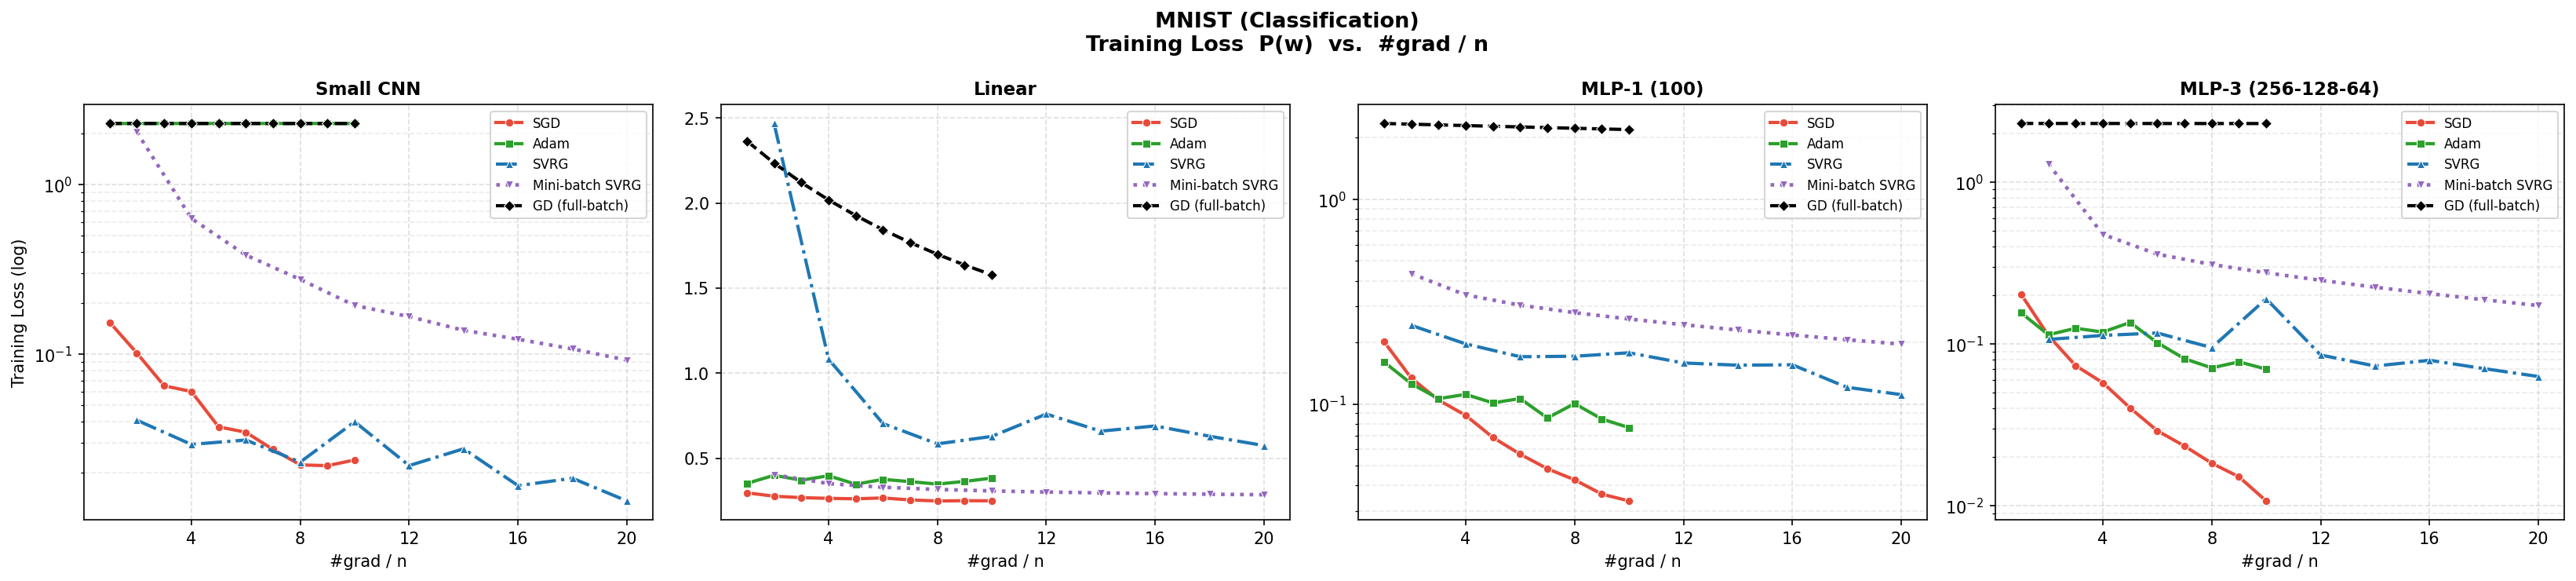
\includegraphics[width=1.0\textwidth]{plots/mnist_1_train_loss_vs_gradn.png}
    \caption{MNIST: Training Loss Comparison}
\end{figure}

\begin{figure}[H]
    \centering
    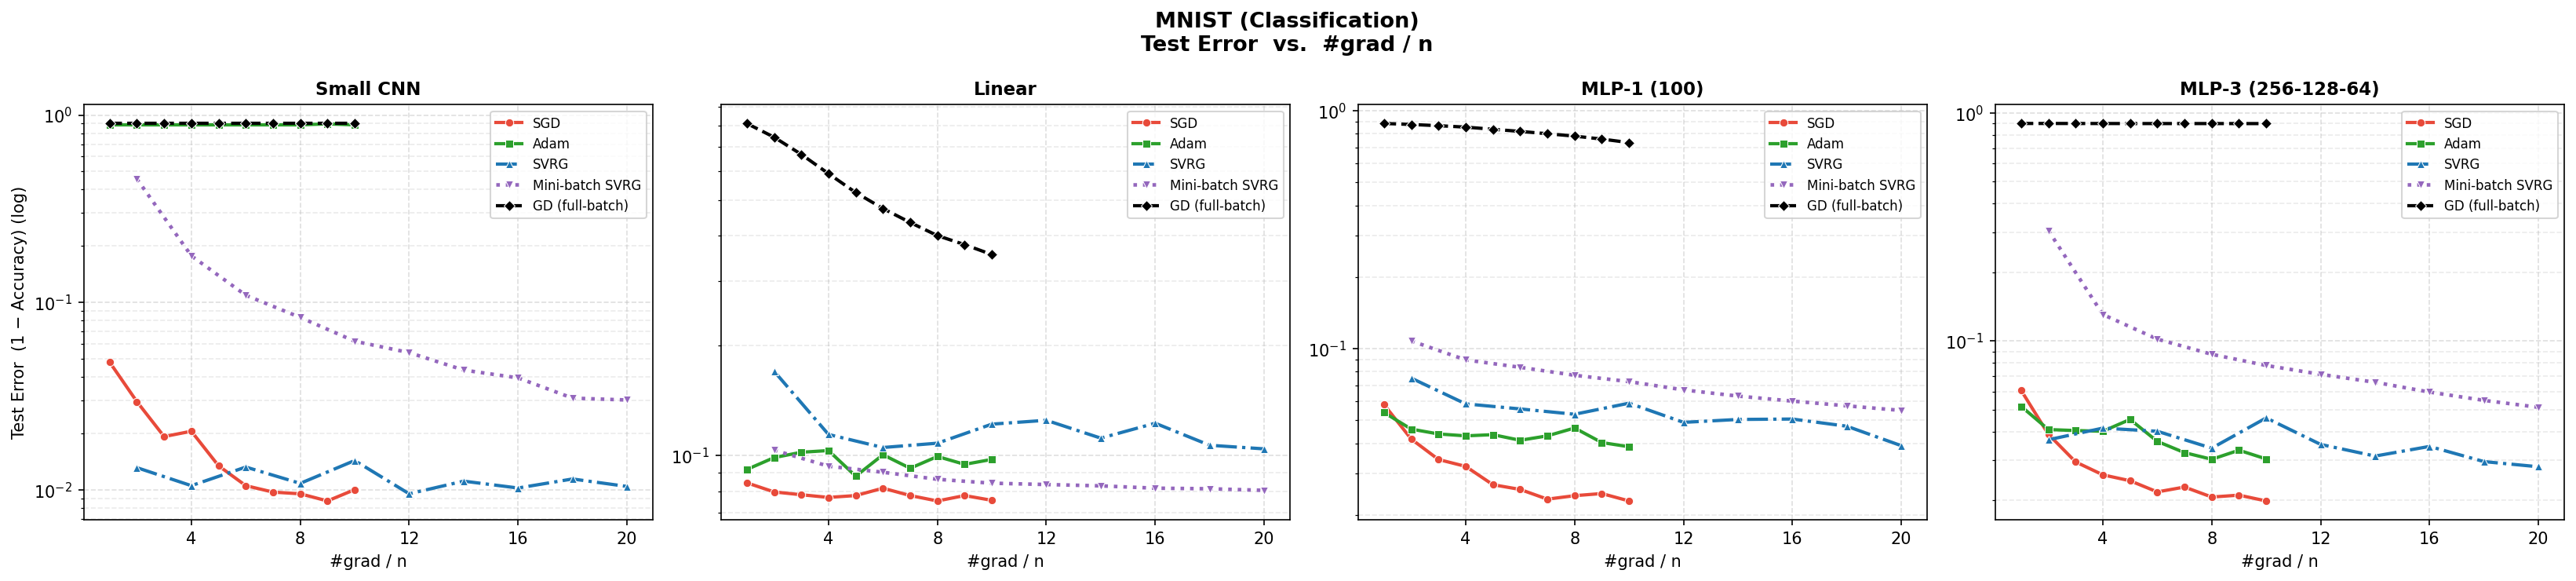
\includegraphics[width=1.0\textwidth]{plots/mnist_2_test_error_vs_gradn.png}
    \caption{MNIST: Test Error (1 - Accuracy) Comparison}
\end{figure}

\begin{figure}[H]
    \centering
    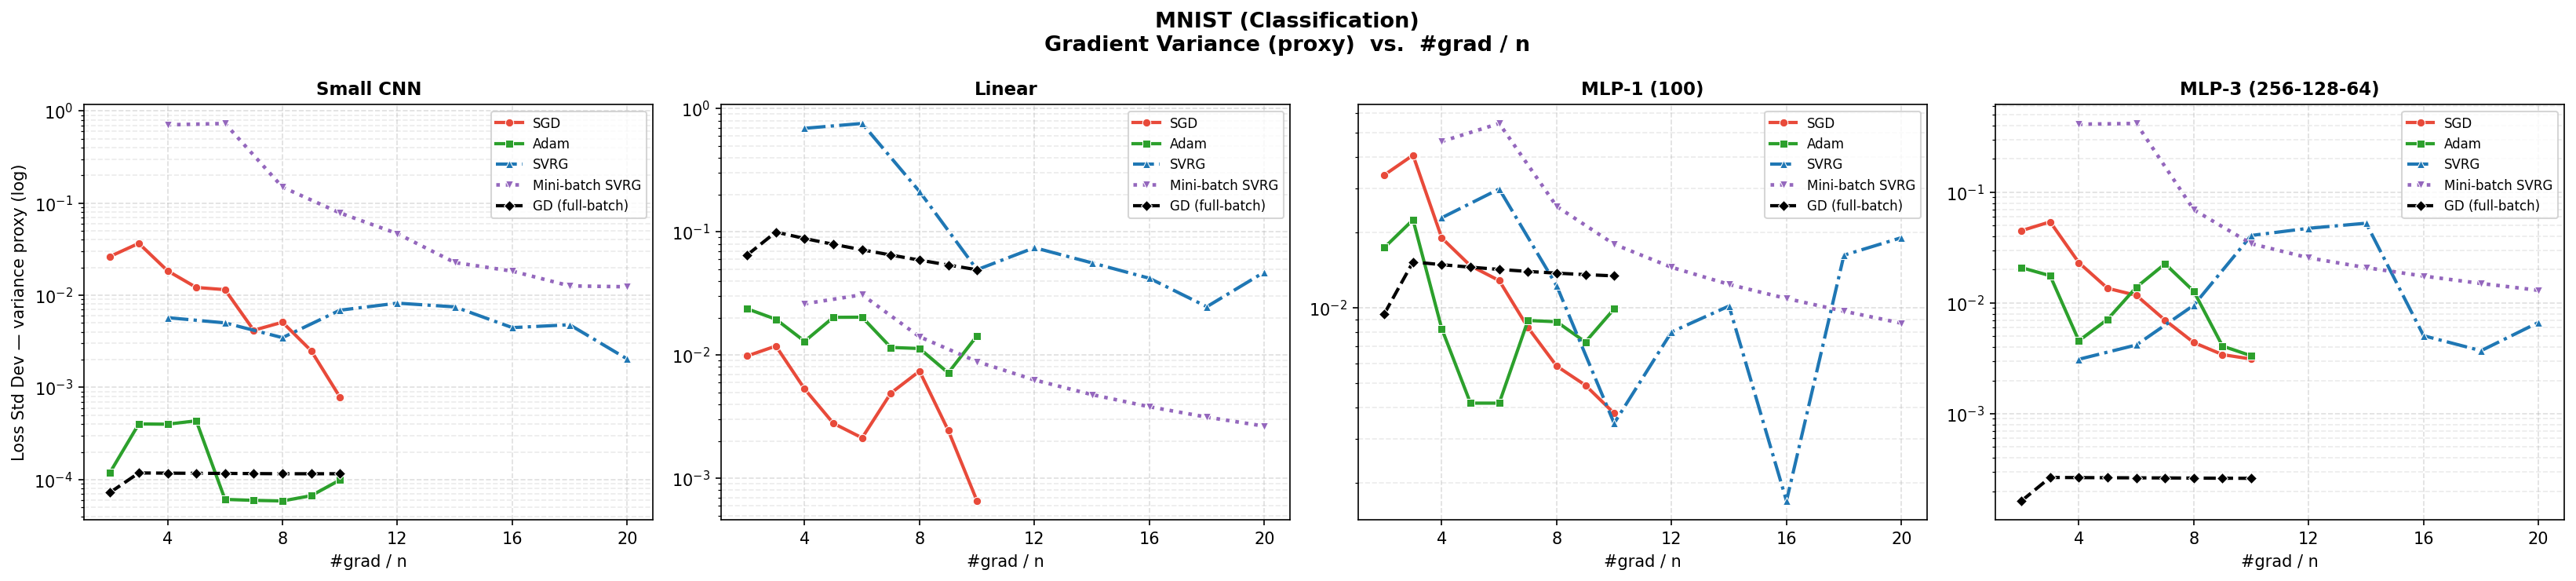
\includegraphics[width=1.0\textwidth]{plots/mnist_3_variance_vs_gradn.png}
    \caption{MNIST: Gradient Variance Proxy Comparison}
\end{figure}

\newpage
\subsection{Mathematical Analysis of MNIST Results}

The MNIST dataset is a standardized image classification task utilizing the Cross-Entropy (CE) loss function. Unlike the unbounded residuals in MSE regression, CE gradients are naturally bounded. This creates a smooth, convex (for the Linear model) or near-convex (for shallow MLPs) loss landscape, completely preventing the catastrophic gradient explosions observed in the California Housing task. As seen in the Training Loss and Test Error plots, all stochastic optimizers successfully converge.

\subsubsection{Successful Variance Reduction in SVRG}
The most distinctive phenomenon occurs in the Gradient Variance Proxy plot. For the Linear and MLP-1 architectures, the variance of standard SVRG (blue) and MB-SVRG (purple) smoothly descends, ultimately dropping significantly below the baseline variance of standard SGD (red). 

Mathematically, this confirms the core theoretical premise of SVRG in well-behaved landscapes. When the objective function is $L$-Lipschitz smooth, the gradients satisfy:
\begin{equation}
\| \nabla \psi_i(w_t) - \nabla \psi_i(\tilde{w}) \|^2 \leq L^2 \| w_t - \tilde{w} \|^2
\end{equation}
Because the CE landscape lacks sharp, erratic curvatures, the fixed learning rate allows the current weights $w_t$ to stay safely within the local vicinity of the snapshot $\tilde{w}$. As the model converges towards the optimum, the physical distance $\| w_t - \tilde{w} \|$ steadily decreases. Consequently, the local stochastic gradient and the snapshot gradient become nearly identical, elegantly canceling out the inherent sampling noise and driving the empirical variance toward zero.

\subsubsection{The Computational Overhead Trade-off}
Despite achieving theoretical variance reduction, both SVRG (blue) and MB-SVRG (purple) noticeably trail behind Adam (green) and SGD (red) along the X-axis (\#grad / n) in both the Training Loss and Test Error plots. 

This visual lag highlights the fundamental computational trade-off of the algorithm. Evaluating the exact full-batch gradient $\tilde{\mu}$ requires a complete pass over the entire dataset ($n=60000$ for MNIST). On the X-axis, this manifests as a flat computational penalty before any parameter updates occur. In highly redundant datasets like MNIST, the stochastic noise of SGD or Adam is already well-aligned with the true gradient direction. Therefore, SVRG pays a massive computational penalty to eliminate a variance component that is not actually detrimental to convergence in this specific, smooth task.

\subsubsection{Adam and SGD Efficiency}
Throughout the plots, Adam (green) exhibits the most rapid initial descent, effectively preconditioning the bounded CE gradients to accelerate through flat regions. Meanwhile, SGD (red) converges reliably with a stable, flat noise floor in the variance plot. The absence of complex, non-convex local minima in MNIST means that Adam's adaptive scaling does not suffer from the severe generalization gap (overfitting to sharp minima) observed in the CIFAR-10 task, allowing both Adam and SGD to reach optimal test accuracy efficiently.

% --- CIFAR-10 Section ---
\newpage
\section{Dataset: CIFAR-10 (Natural Image Classification)}
CIFAR-10 involves a highly non-convex loss landscape. It is used to evaluate the robustness and generalization capabilities of optimizers in deep learning scenarios.

\begin{figure}[H]
    \centering
    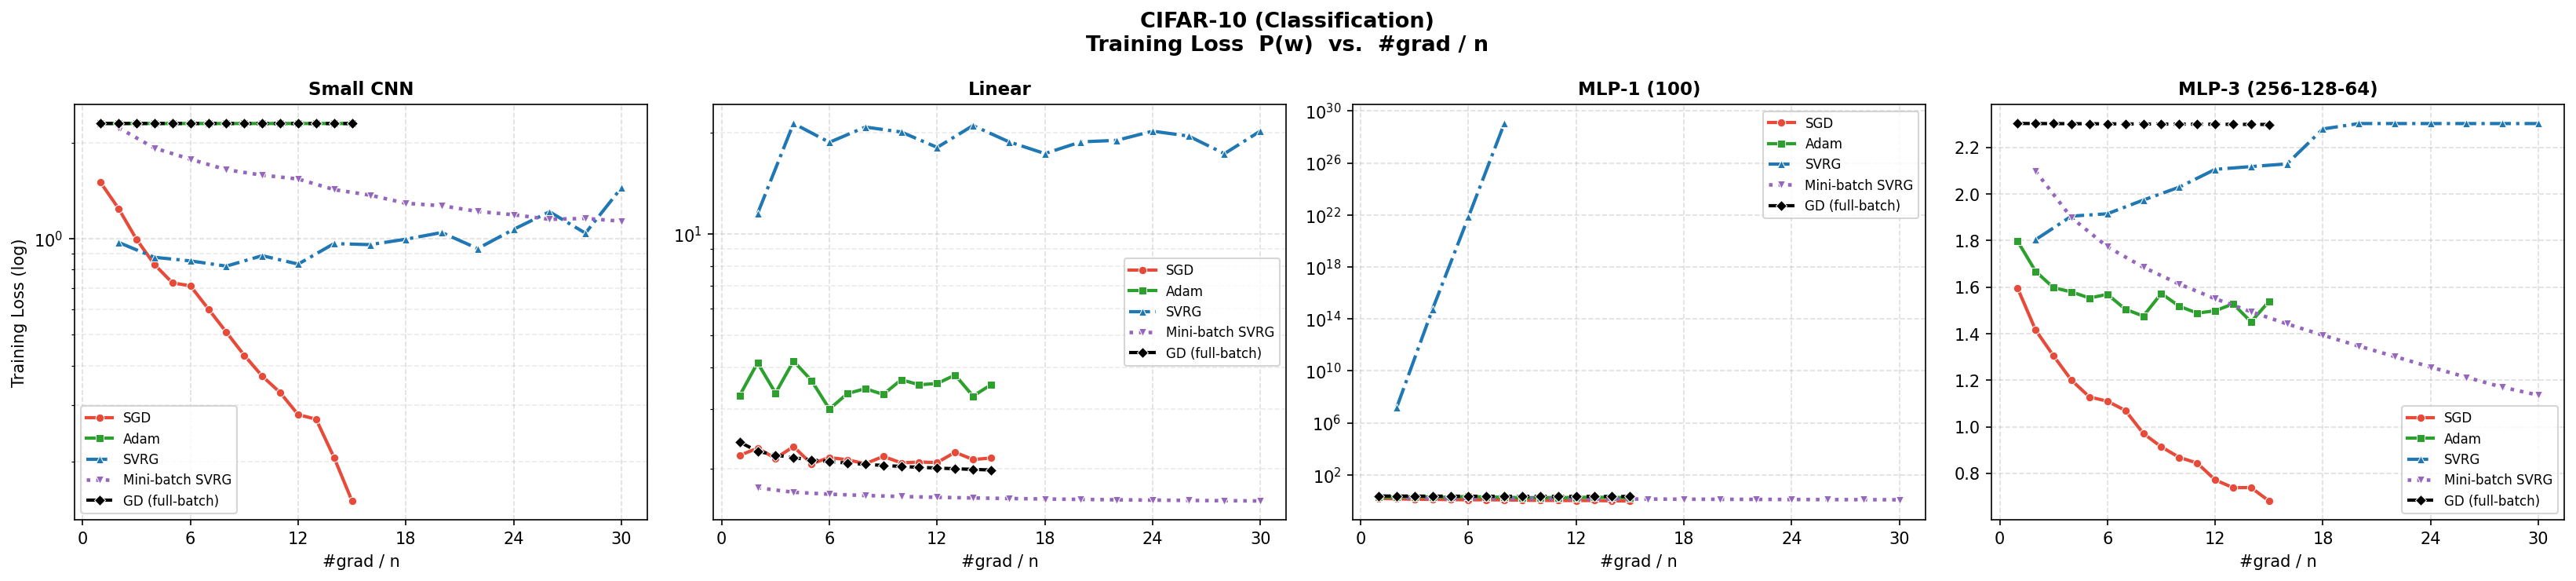
\includegraphics[width=1.0\textwidth]{plots/cifar10_1_train_loss_vs_gradn.png}
    \caption{CIFAR-10: Training Loss Comparison}
\end{figure}

\begin{figure}[H]
    \centering
    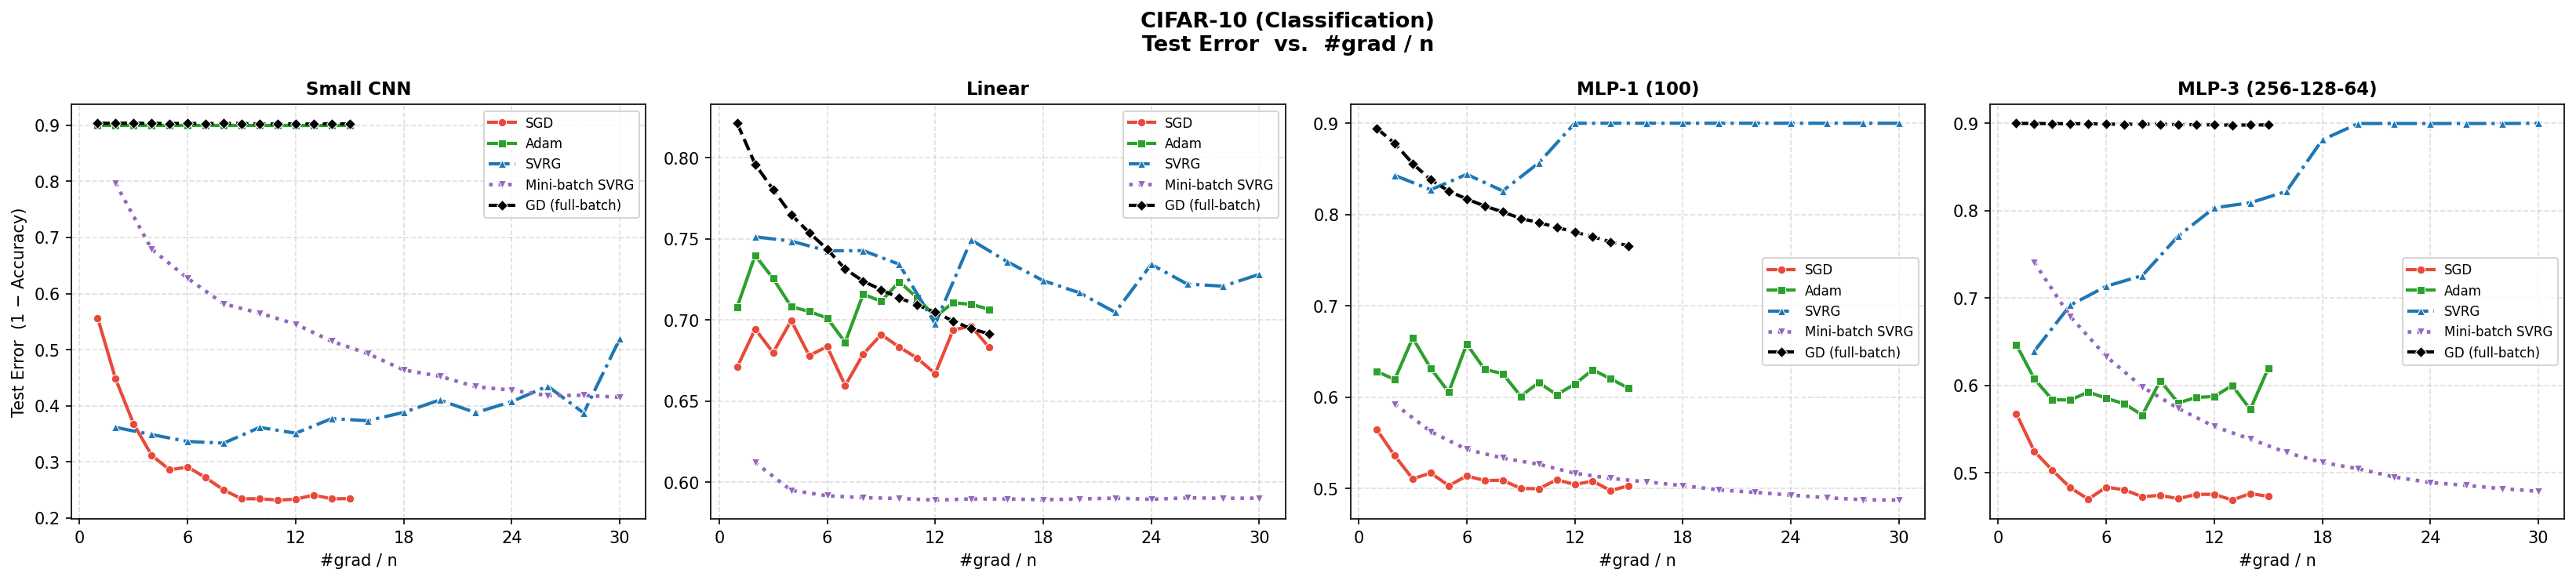
\includegraphics[width=1.0\textwidth]{plots/cifar10_2_test_error_vs_gradn.png}
    \caption{CIFAR-10: Test Error Comparison}
\end{figure}

\begin{figure}[H]
    \centering
    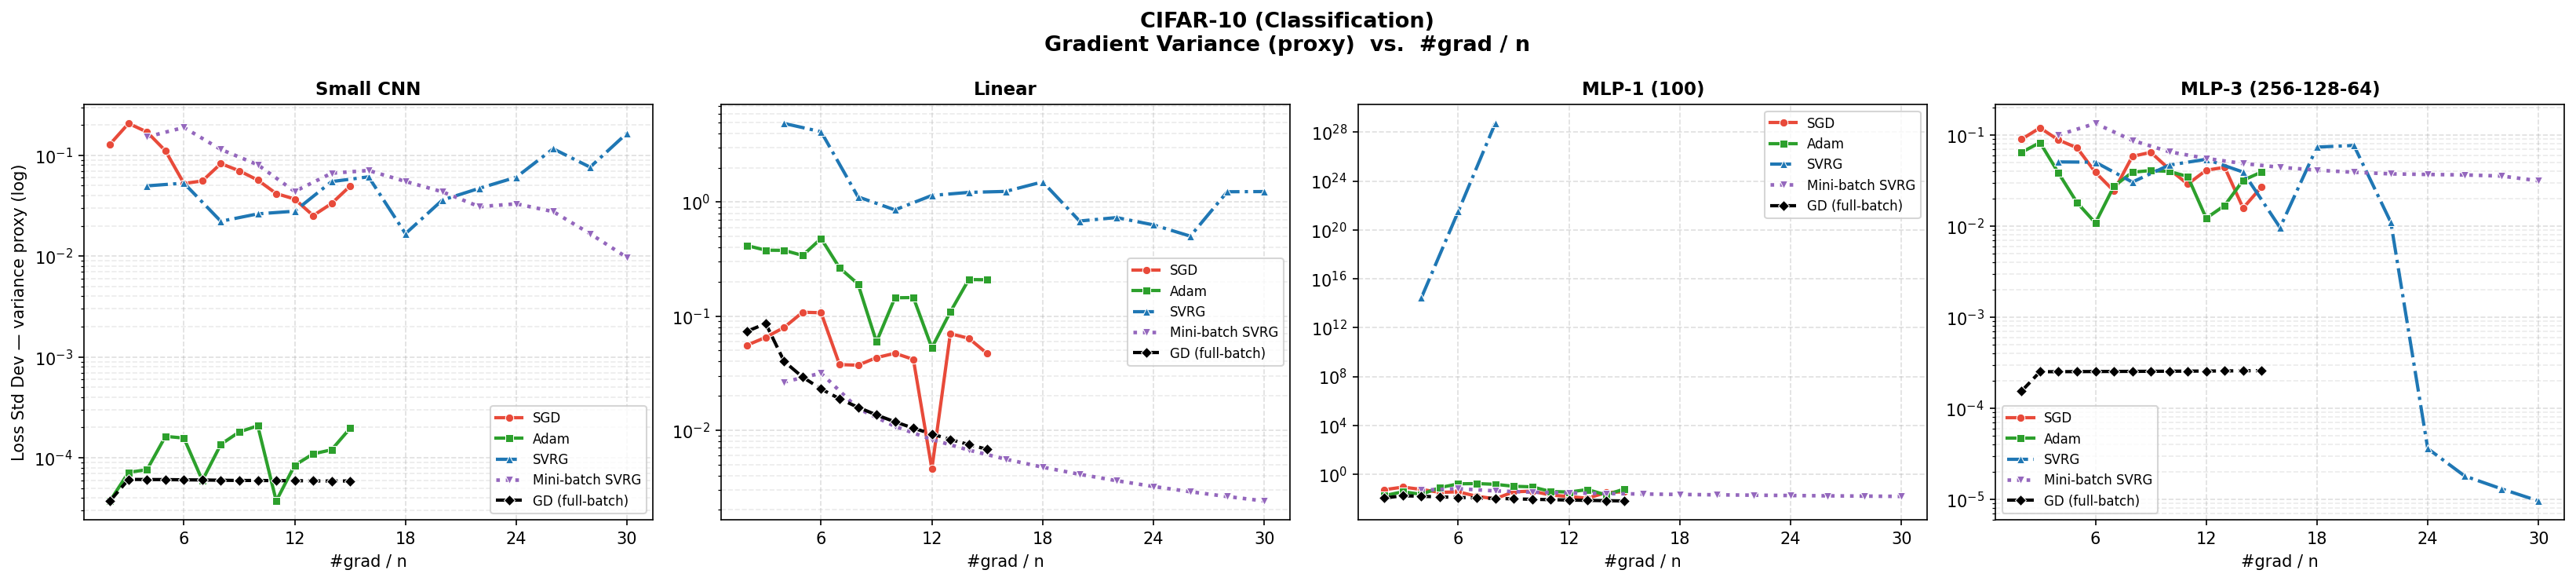
\includegraphics[width=1.0\textwidth]{plots/cifar10_3_variance_vs_gradn.png}
    \caption{CIFAR-10: Gradient Variance Proxy Comparison}
\end{figure}

\newpage
\subsection{Mathematical Analysis of CIFAR-10 Results}

The CIFAR-10 dataset presents a highly complex, non-convex image classification task. While it uses the Cross-Entropy loss where gradients are inherently bounded (unlike the regression task), the primary optimization challenge stems from navigating the highly non-linear and sharp loss landscapes associated with deeper architectures like MLP-3 and Small CNN.

\subsubsection{SVRG Breakdown in Non-Convex Landscapes}
In the Training Loss plot, we observe that standard SVRG (blue) completely diverges in the MLP-3 and Small CNN architectures, shooting upwards on the log scale. Concurrently, in the Gradient Variance plot, its variance proxy explodes to the $10^4$ range. Mathematically, SVRG relies on the snapshot gradient $\nabla P(\tilde{w})$ acting as a reliable anchor. A Taylor expansion of the full gradient illustrates the local geometry:
\begin{equation}
\nabla P(w_t) \approx \nabla P(\tilde{w}) + \nabla^2 P(\tilde{w})(w_t - \tilde{w})
\end{equation}
where $\nabla^2 P(\tilde{w})$ is the Hessian matrix. In deep, non-convex neural networks, the Hessian changes abruptly over very short distances in the parameter space. Taking just a few update steps causes the linear approximation to fail. Consequently, the snapshot $\tilde{w}$ becomes critically "stale." Subtracting this stale gradient no longer reduces variance; instead, it injects severe, directionless noise that forcefully ejects the weights from viable local valleys, causing the observed explosion.

\subsubsection{The Generalization Gap (SGD vs. Adam)}
Comparing the Training Loss and Test Error plots for the Small CNN reveals a profound generalization gap: while Adam (green) minimizes the training loss much faster and reaches a lower floor, SGD (red) ultimately achieves a lower Test Error, crossing under Adam after a few effective passes. Mathematically, SGD introduces inherent stochastic gradient noise $\xi_t = \nabla \psi_{i_t}(w_t) - \nabla P(w_t)$. Its update rule can be rewritten as:
\begin{equation}
w_{t+1} = w_t - \eta \nabla P(w_t) + \eta \xi_t
\end{equation}
This isotropic noise acts as an implicit regularization mechanism. Adam's adaptive scaling aggressively preconditions the gradients, allowing it to rapidly descend into the nearest local minimum, which is often sharp and prone to overfitting. In contrast, the continuous "jiggling" force from $\eta \xi_t$ prevents SGD from settling into these narrow, sharp valleys. It is mathematically forced to escape and settle into wider, flatter minima. Flat minima provide a wider margin for error against unseen data, directly explaining SGD's superior test accuracy.

\subsubsection{Variance Proxy and MB-SVRG Survival}
In the Gradient Variance Proxy plot, while standard SVRG explodes, MB-SVRG (purple) manages to survive the non-convex topography, though it maintains a high variance and converges slower than Adam or SGD. By substituting the single-sample gradient with a mini-batch gradient $\frac{1}{|B|} \sum_{j \in B} \nabla \psi_j(w)$, the variance of the local update is reduced by a factor of the batch size $|B|$. This mini-batch averaging acts as a critical buffer against the catastrophic "stale snapshot" noise injection described above. However, because the underlying Hessian still shifts rapidly, the core assumption of SVRG remains violated, explaining why MB-SVRG barely survives but fails to achieve the theoretical variance reduction (towards zero) seen in simpler tasks.

\newpage
\section{Conclusion}

Based on the experiments across the California Housing, MNIST, and CIFAR-10 datasets, we can draw the following practical conclusions:

\begin{enumerate}
    \item \textbf{Adam's Robustness:} Adam remains highly stable across all tasks. Its adaptive learning rate effectively handles both the exploding gradients in regression tasks and the highly non-convex loss surfaces of deep CNNs, succeeding where other optimizers diverge.
    
    \item \textbf{SVRG's Computational Cost:} In simple, smooth tasks like MNIST, SVRG successfully reduces gradient variance. However, constantly computing the full-dataset snapshot is computationally expensive. When measured by actual gradient computations (\#grad/n), standard SGD and Adam are practically much faster.
    
    \item \textbf{SVRG Fails in Deep Learning:} In complex architectures like CIFAR-10 CNNs, the loss surface changes too rapidly. SVRG's gradient snapshot becomes stale almost instantly, injecting outdated noise into the updates and causing divergence. While mini-batches (MB-SVRG) cushion this effect, they still fail to reduce variance effectively.
    
    \item \textbf{SGD Generalizes Better:} While Adam minimizes training loss faster, SGD achieves lower test errors on complex tasks like CIFAR-10. The inherent noise in SGD prevents it from getting trapped in sharp training valleys, helping the model find flatter minima that generalize better to unseen data.
\end{enumerate}

\end{document}